%!TeX spellcheck = es_ES
%!TEX program = lualatex
\documentclass[hyperref={unicode}]{beamer}

\usepackage[spanish]{babel}
\usepackage{graphicx}
\usepackage[unicode]{hyperref}
\usepackage{bookmark}
\usepackage{tikz}
\usepackage{etoolbox}



\usetheme{TFM}

\title{Título del TFM}
\subtitle{Trabajo Fin de Máster \\ \textbf{Máster en Ingeniería de Sistemas de Decisión} \\ \textit{Curso 2016--2017}}
\author{José Ignacio Escribano Pablos}
\institute{Ana Elizabeth García Sipols \\ Miguel Romance del Río}
\titlegraphic{
\includegraphics[width=2cm]{imagenes/urjc.png}}

\setcounter{tocdepth}{2}

\makeatletter
\patchcmd{\beamer@sectionintoc}
{\vfill}
{\vskip\itemsep}
{}
{}
\makeatother  


\setcounter{showSlideNumbers}{1}

\begin{document}
\setcounter{showProgressBar}{0}
\setcounter{showSlideNumbers}{0}

\frame{\titlepage}

\begin{frame}{Índice}
	\tableofcontents
\end{frame}

\setcounter{framenumber}{0}
\setcounter{showProgressBar}{1}
\setcounter{showSlideNumbers}{1}
\section{Introducción}
\begin{frame}{Objetivos}
	\begin{enumerate}
		\item Introducir los conceptos básicos de Machine Learning, teoría de grafos y redes parenclíticas (basadas en grafos).
		
		\item \pause Desarrollar una aplicación que automatice el proceso del aprendizaje según los distintos algoritmos de Machine Learning anteriores.
		
		\item \pause Analizar una base de datos y comparar los resultados de los distintos algoritmos de Machine Learning.
	\end{enumerate}
\end{frame}

\begin{frame}{Introducción}
	\Huge{\textcolor{red}{TODO}}
\end{frame}

\section{Introducción al Machine Learning}
\begin{frame}{Definición de Machine Learning}
	\begin{fancyquotes}
		Machine learning, in artificial intelligence (a subject within computer science), discipline concerned with the implementation of computer software that can learn autonomously.
	\end{fancyquotes}
\end{frame}

\subsection{Problemas que resuelve}
\begin{frame}{Problemas que resuelve}
Regresión y clasificación
Poner imágenes
\end{frame}

\subsubsection{Regresión}
\begin{frame}{Regresión}
	
\end{frame}

\begin{frame}{Regresión lineal}
	
\end{frame}

\subsubsection{Clasificación}
\begin{frame}{Clasificación}
	
\end{frame}

\subsection{Tipos de aprendizaje}
\subsubsection{Aprendizaje supervisado}
\begin{frame}{Aprendizaje supervisado}
	
\end{frame}

\begin{frame}{Proceso}
	Proceso
\end{frame}

\begin{frame}{Aplicaciones}
	Aplicaciones aprendizaje supervisado
\end{frame}

\subsubsection{Aprendizaje no supervisado}
\begin{frame}{Aprendizaje no supervisado}
	
\end{frame}

\begin{frame}{Aplicaciones}
	Aplicaciones aprendizaje no supervisado
\end{frame}

\subsubsection{Aprendizaje por refuerzo}
\begin{frame}{Aprendizaje por refuerzo}
	
\end{frame}

\begin{frame}{Aplicaciones}
	Aplicaciones aprendizaje por refuerzo
\end{frame}

\section{Redes parenclíticas}
\begin{frame}{Redes parenclíticas}
	
\end{frame}

\subsection{Introducción a la teoría de grafos}
\begin{frame}{Introducción a la teoría de grafos}
	
\end{frame}

\subsection{Medidas de redes complejas}
\begin{frame}{Medidas de redes complejas}
	
\end{frame}

\subsection{Descripción del método de redes parenclíticas}
\begin{frame}{Método de redes parenclíticas}
	
\end{frame}

\section{Diseño de la aplicación}
\begin{frame}{Diseño de la aplicación}
	
\end{frame}

\begin{frame}{Arquitectura}
	Arquitectura
\end{frame}

\begin{frame}{Tecnología}
	Tecnología
\end{frame}

\begin{frame}{Vista de la aplicación}
	[DEMO]
\end{frame}

\section{Aplicación al cáncer de mama}
\begin{frame}{Aplicación al cáncer de mama}
	Aplicación al cáncer de mama
\end{frame}

\section{Conclusiones y trabajo futuro}
\begin{frame}{Conclusiones}
	Conclusiones
\end{frame}

\begin{frame}{Trabajo futuro}
	Trabajo futuro
\end{frame}

\begin{frame}{¿Preguntas?}
	
	{%
		\centering
		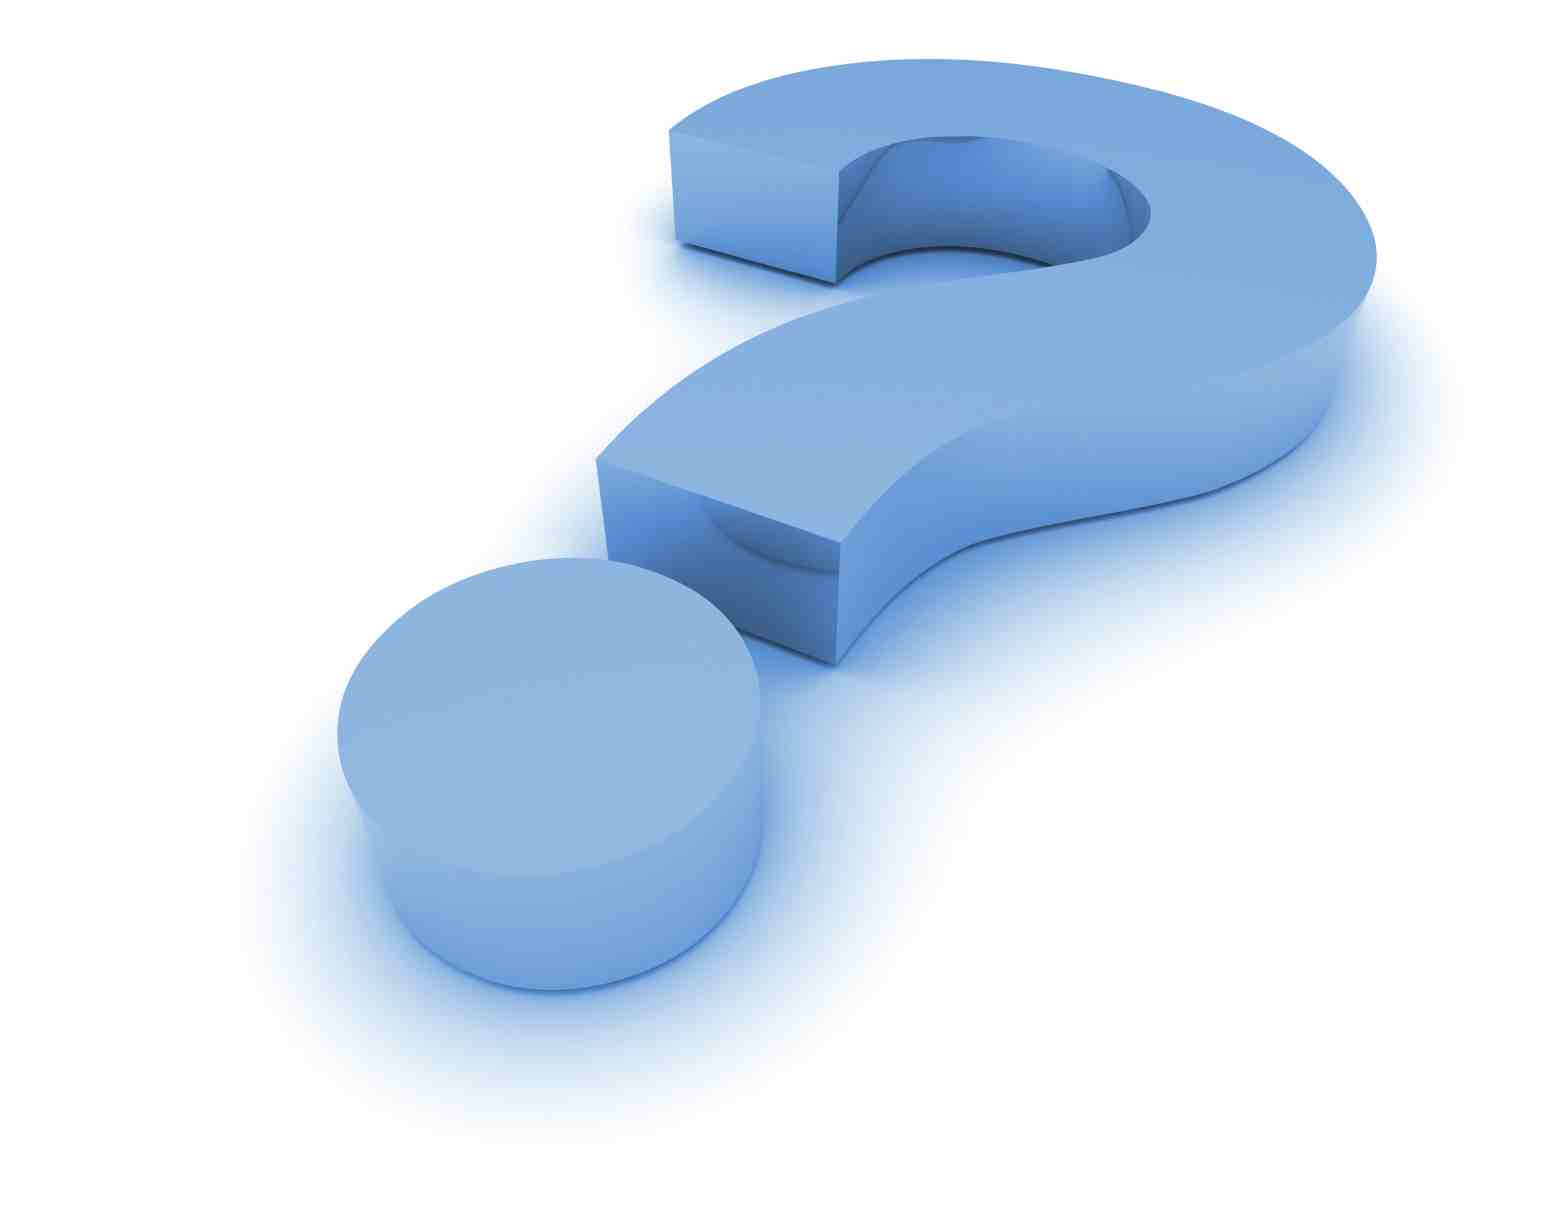
\includegraphics[width=0.8\textwidth]{imagenes/questions}
	}


\end{frame}

\end{document}